\documentclass[UTF8]{scrartcl}

\usepackage{xeCJK}
\usepackage{graphicx}
\usepackage{subfigure}
\usepackage{indentfirst}
\setlength{\parindent}{2em}

%opening
\title{A Polyhedral-based SystemC Modeling and Generation Framework for Effective Low-power Design Space Exploration}
\author{}

\begin{document}

\maketitle

\begin{abstract}

\end{abstract}

\section{Introduction}
	
	对于整个Soc的建模,业界已转向使用高层硬件描述,TLM(transaction level)的SystemC广泛使用。在传统的设计流程中,the SoC design specification is often provided in a high level language such as C/C++ by software engineers as a golden reference model,然后手工进行软硬划分并编写systemC描述的硬件代码。这样的流程有以下弊端:1. 硬件部分的system实现需要additional effort; 2. SystemC model是手工实现的,难以有效和extensively探索不同的设计选择; 3. 这一阶段由于缺少低层次的实现细节,难以获得精确的能耗估计; 4. SystemC IP一般考虑仿真速度、复用等,不一定可以作为HLS的输入去综合; 5. System C model只能提供一个design point的仿真,整个空间太大了。
	
	本文提出了自动化设计流程来解决上述问题,针对的是the class of affine programs,例如图像处理、医学影像、统计等。这一类程序的一个特点是having a control-flow that can be exactly described at compile-time [4] thereby allowing the design of accurate power/latency models, and very powerful optimization frameworks to expose parallelism with data reuse that have already been developed。输入是C++应用,可以自动提取出affine program的区域,并自动化执行三个操作:自动进行software transformation,体现并行度和temporal data locality。自动生成两个版本的System C,一个包括power和latency的高层模型用,一个用于HLS的可综合的systemC。自动实现一个DSE engine,考虑了不同的loop tile sizes和parallism degree。


\section{SystemC Generation Framework}

	\subsection{Overview}

		相比较之前的工作,该framework的特点有以下几点:使用了Polyopt compilation framework。生成communication and computation blocks并建立对应的power、latency模型,考虑了开关活性、加速器与系统的交互等因素。latency和power的characterization是针对1个tile,可以借助polyopt分析。	相比较functional level的功耗分析,tile-based可以更方便地使用IP、blackbox在设计中。	快速仿真,使用行为级的systemC。
		
		整个流程如下图所示,首先将输入的program转化成可以做loop tile的形式并使用Polyopt来tile loop。之后,将tile提取出来,分成不同的部分包括计算block和通信block,后者在tile的开始或结束负责把memory和local buffer之间的数据移动。下一阶段,借助gate-level的仿真characterize这些block建立power和latency,并建立功耗模型。最后借助polyhedral analysis,为tiled loop kernel生成systemC模型并将power和latency的模型加进去。
		
			\begin{figure}[h]
				\centering
				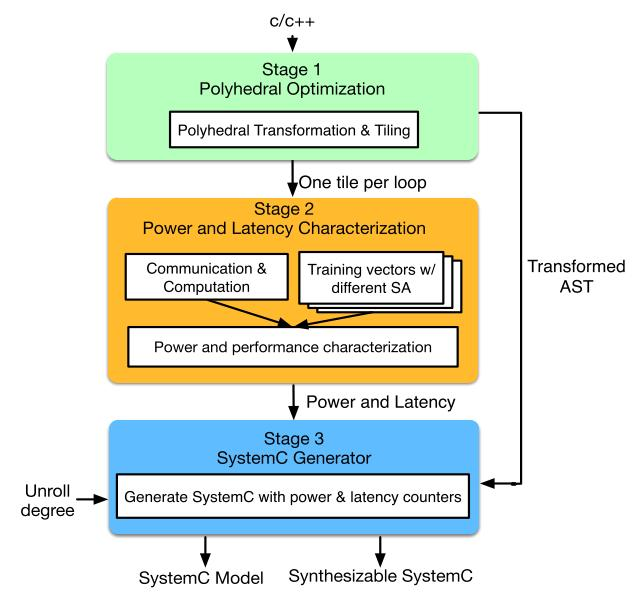
\includegraphics[width=4.00in,height=3.50in]{system.jpg} 
				\caption{系统流程}
				\label{fig1}
			\end{figure}

	\subsection{Architecture of Generated Accelerator}
		
		生成的加速器架构基本结构如下图所示,包括计算模块(Acc\_tile)和片内存储(Local\_mem)。计算模块负责从local\_mem中读取数据并计算和写回,而communication blocks负责local\_mem和main\_mem之间的数据交换。有两个可控制参数,一是tile size,影响loop tiling的选择、buffer size以及相应通信消耗;二是parallelism degree,决定哪一个层次的循环被展开; 这两个因素决定了tile的重复单元个数。此外,在每个block中实现了一个input switching activity calculation function,用以分析使用活性。(利用率?)
		
		\begin{figure}[h]
			\centering
			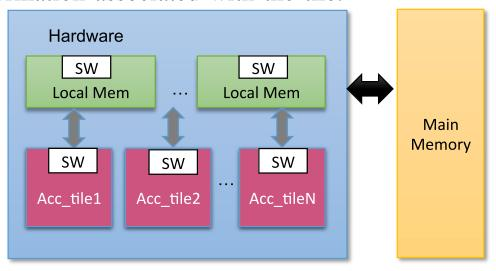
\includegraphics[width=3.50in,height=2.00in]{hardware.jpg} 
			\caption{硬件架构示意图}
			\label{fig2}
		 \end{figure}
		
	\subsection{Software Transformation}
		
		软件转换有3个要求:(1)要体现temporal data locality来减少数据移动; (2)要体现并行性; (3)explicit atomic computation tiles and the associated tile data reuse buffers and data transfers operations(这一点还不太理解); 但所有这些都可以借助Polyopt实现。
		
	\subsection{Power and Latency Characterization}
	
		这一部分关注单独的tile,把一个tile的computation block输入HLS和Memory Compiler分别生成RTL code和local mem。这两部分结合起来做逻辑综合生成网表,并进行门级仿真,然后提取power和latency的信息。计算部分有loop unroll和pipeline的考虑,对于communication block,生成一个memory Ip库(with 不同size)并根据不同的开关活性提取power和latency信息组成查找表。
		此外,也会生成testbench和input vectors。后者的开关活性可控,服从一定分布等。功耗有三部分:internal, switching and leakage power,前两个动态功耗,分别由capacitive charging/discharging of output load and internal transistors of the logic gates导致,最后一个是静态功耗。
	
	\subsection{SystemC Code Generation}
	
		high-level model: 每一个tile生成systemC中的module,wait()来模拟function module的latency,power信息根据不同的开关活性从power model中索引。switching activity calculation function没看太明白。
		
		synthesizable version: 可综合的版本有三个调整:1.要解决访存冲突;2. 要解决同一存储地址的read/write 冲突; 3. 移除high-level模型中的latency和power的函数。
	
	\subsection{Integration}
		
		生成SystemC并将一个tile的power和latency信息加入后,可以做快速的systemC仿真(使用的就是SystemC 仿真)。latency通过在每一个tile中插入的systemC wait()函数来计算。功耗通过插入monitor函数,在每一个tile module开始和结束式调用update\_power( )来计算功耗,根据wait( )计算执行时间提供信息。 Power和latency都是分别考虑computation blocks和communication blocks,不同的tile构成系统时,由于是重复的调用且并行的tile是复制的,因此当系统启动和同步等一些操作的overhead可忽略时,系统的power和latecy是这些tile的求和,具体计算时会考虑动态功耗、静态功耗差异、开关活性、tile size、unroll factor等信息。

\end{document}
